\documentclass[__main__.tex]{subfiles}

\begin{document}

\qtitle{Э}{13}
Воспользуйтесь законом Био-Савара-Лапласа, чтобы вычислить магнитное поле прямого постоянного тока $I$ на расстоянии $R$ от него. Проверьте результат с помощью теоремы о циркуляции $\vec{B}$.\\ 

\textbf{Закон Био - Савара}

	Рассмотрим вопрос о нахождении магнитного поля, создаваемого постоянными электрическими токами. Этот вопрос будем решать, исходя из закона 
	\begin{gather}
	\llabel{y1}
	\vec{B} = \frac{\mu_0}{4\pi} \frac{q[\vec{v},\vec{r}]}{r^3},
	\end{gather}
	который определяет индукцию поля $\vec{B}$ равномерно  движущегося точеченого заряда. Подставим в \lref{y1} вместо $q$ заряд $\rho dV$, где $dV$ - элементарный объём, $\rho$ - объёмная плотность заряда, являющегося носителем тока и учтём, что $\rho \vec{v} = \vec{j}$ согласно определению вектора плотности тока. Тогда формула \lref{y1} приобретёт следующий вид:
	
	\begin{gather}
	\llabel{y2}
	d\vec{B}= \frac{\mu_0}{4\pi} \frac{[\vec{j},\vec{r}] dV}{r^3}.
	\end{gather}
	
	Если же ток $I$ течёт по тонкому проводу с площадью поперечного сечения $\Delta S$, то 
	
	$$j dV = d \Delta S dl = l dl,$$
	
	где $dl$ - элемент длины провода. Введя векктор $d\vec{l}$ в направлении тока $I$, перепишем предыдущее равенство так:
	
	$$j dV = I d\vec{l}.$$
	
	Векторы $\vec{j} dV$ и $I d\vec{l}$ называются соответственно \textit{объёмным и линейным элементами тока}. Произведя в формуле \lref{y2} замену объёмного элемента тока на линейный получим
	
	\begin{gather}
	\llabel{y3}
		d\vec{B} = \frac{\mu_0}{4\pi} \frac{I[d\vec{l},\vec{r}]}{r^3}
	\end{gather}
	
	Формулы \lref{y2} и \lref{y3} выражают \textit{закон Био-Савара}.
	
	Полное поле $\vec{B}$ в соответствии с принципом суперпозиции определяется в результате интегрирования выражений \lref{y2} или \lref{y3} по всем элементам тока:
	
	$$\vec{B} = \frac{\mu_0}{4\pi} \int \frac{[\vec{j},\vec{r}]}{r^3}, \ \ \ \vec{B} = \frac{\mu_0}{4\pi}\oint \frac{I[d\vec{l},\vec{r}]}{r^3} $$
	
	
	
	\textbf{Теорема о циркуляции вектора $\vec{B}$}
	Циркуляция вектора $\vec{B}$ по произвольному контуру $\Gamma$ равна произведению $\mu_0$ на алгебраическую сумму токов, охватываемых контуром $\Gamma$:
	
	\begin{gather}
	\oint \vec{B} d\vec{l} = \mu_0 I,
	\end{gather}
	
	где $I = \sum I_k$.\\
	
	\textbf{Перейдём к решению задачи:}
	
	\begin{center}
		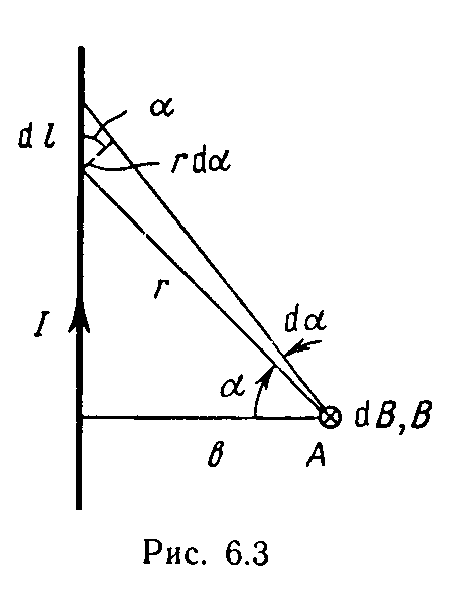
\includegraphics[]{e-13_1.png}
	\end{center}

	Согласно \lref{y3} в произвольной точке А векторы $d\vec{B}$ от всех элементов тока имеют одинаковое направление - за плоскость рисунка. Поэтому сложение векторов $d\vec{B}$ можно заменить сложением их модулей $dB$, причём
	
	$$dB = \frac{\mu_0}{4\pi} \frac{I dl \cos \alpha}{r^2}.$$
	
	Из рисунка видно, что $dl \cos \alpha = r d\alpha$ и $r = \frac{b}{\cos \alpha}$. Поэтому 
	
	$$dB = \frac{\mu_0}{4\pi} \frac{I \cos \alpha d\alpha}{b}.$$
	
	Интегрируя последнее выражение по всем элементам тока, что эквивалентно интегрированию по $\alpha$ от $-\frac{\pi}{2}$ до $\frac{\pi}{2}$, находим
	
	$$B = \frac{\mu_0}{4\pi} \frac{2I}{b}.$$
	
	(Только теперь везде надо учесть, что $b = R$ по условию)
	
	\textbf{Теперь решим ту же задачу с помощью теоремы о циркуляции:}
	
	\begin{center}
		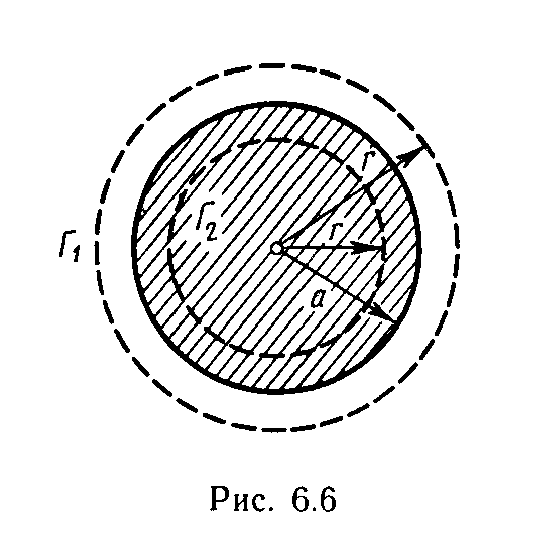
\includegraphics[]{e-13_2.png}
	\end{center}

	Из симметрии задачи следует, что линии вектора $\vec{B}$ в заданном случае должны иметь вид окружностей с центром на оси провода. Причём модуль вектора $\vec{B}$ должен быть одинаков во всех точках на расстоянии $R$ от оси провода. Поэтому по теореме о циркуляции вектора $\vec{B}$ для круглого контура $\Gamma_1$ получим $2 \pi R B = \mu_0 I,$ откуда следует, что вне провода
	
	$$B = \frac{\mu_0}{2 \pi} \frac{I}{R}.$$
	
	\textbf{В итоге получили, что решения через закон Био-Савара и теорему о циркуляции $\vec{B}$ равны.}
%%

\end{document}